
% Inherit from the specified cell style.

% Default to the notebook output style

    


% Inherit from the specified cell style.




    
\documentclass[letter]{article}

    
    
% \usepackage{stix}
\usepackage[scr]{rsfso}
\usepackage{bm}

    \usepackage[T1]{fontenc}
    % Nicer default font than Computer Modern for most use cases
    \usepackage{palatino}

    % Basic figure setup, for now with no caption control since it's done
    % automatically by Pandoc (which extracts ![](path) syntax from Markdown).
    \usepackage{graphicx}
    % We will generate all images so they have a width \maxwidth. This means
    % that they will get their normal width if they fit onto the page, but
    % are scaled down if they would overflow the margins.
    \makeatletter
    \def\maxwidth{\ifdim\Gin@nat@width>\linewidth\linewidth
    \else\Gin@nat@width\fi}
    \makeatother
    \let\Oldincludegraphics\includegraphics
    % Set max figure width to be 80% of text width, for now hardcoded.
    \renewcommand{\includegraphics}[1]{\Oldincludegraphics[width=.8\maxwidth]{#1}}
    % Ensure that by default, figures have no caption (until we provide a
    % proper Figure object with a Caption API and a way to capture that
    % in the conversion process - todo).
    \usepackage{caption}
    \DeclareCaptionLabelFormat{nolabel}{}
    \captionsetup{labelformat=nolabel}

    \usepackage{adjustbox} % Used to constrain images to a maximum size 
    \usepackage{xcolor} % Allow colors to be defined
    \usepackage{enumerate} % Needed for markdown enumerations to work
    \usepackage{geometry} % Used to adjust the document margins
    \usepackage{amsmath} % Equations
    \usepackage{amssymb} % Equations
    \usepackage{textcomp} % defines textquotesingle
    % Hack from http://tex.stackexchange.com/a/47451/13684:
    \AtBeginDocument{%
        \def\PYZsq{\textquotesingle}% Upright quotes in Pygmentized code
    }
    \usepackage{upquote} % Upright quotes for verbatim code
    \usepackage{eurosym} % defines \euro
    \usepackage[mathletters]{ucs} % Extended unicode (utf-8) support
    \usepackage[utf8x]{inputenc} % Allow utf-8 characters in the tex document
    \usepackage{fancyvrb} % verbatim replacement that allows latex
    \usepackage{grffile} % extends the file name processing of package graphics 
                         % to support a larger range 
    % The hyperref package gives us a pdf with properly built
    % internal navigation ('pdf bookmarks' for the table of contents,
    % internal cross-reference links, web links for URLs, etc.)
    \usepackage{hyperref}
    \usepackage{longtable} % longtable support required by pandoc >1.10
    \usepackage{booktabs}  % table support for pandoc > 1.12.2
    \usepackage[normalem]{ulem} % ulem is needed to support strikethroughs (\sout)
                                % normalem makes italics be italics, not underlines
    


    
    
    
    % Colors for the hyperref package
    \definecolor{urlcolor}{rgb}{0,.145,.698}
    \definecolor{linkcolor}{rgb}{.71,0.21,0.01}
    \definecolor{citecolor}{rgb}{.12,.54,.11}

    % ANSI colors
    \definecolor{ansi-black}{HTML}{3E424D}
    \definecolor{ansi-black-intense}{HTML}{282C36}
    \definecolor{ansi-red}{HTML}{E75C58}
    \definecolor{ansi-red-intense}{HTML}{B22B31}
    \definecolor{ansi-green}{HTML}{00A250}
    \definecolor{ansi-green-intense}{HTML}{007427}
    \definecolor{ansi-yellow}{HTML}{DDB62B}
    \definecolor{ansi-yellow-intense}{HTML}{B27D12}
    \definecolor{ansi-blue}{HTML}{208FFB}
    \definecolor{ansi-blue-intense}{HTML}{0065CA}
    \definecolor{ansi-magenta}{HTML}{D160C4}
    \definecolor{ansi-magenta-intense}{HTML}{A03196}
    \definecolor{ansi-cyan}{HTML}{60C6C8}
    \definecolor{ansi-cyan-intense}{HTML}{258F8F}
    \definecolor{ansi-white}{HTML}{C5C1B4}
    \definecolor{ansi-white-intense}{HTML}{A1A6B2}

    % commands and environments needed by pandoc snippets
    % extracted from the output of `pandoc -s`
    \providecommand{\tightlist}{%
      \setlength{\itemsep}{0pt}\setlength{\parskip}{0pt}}
    \DefineVerbatimEnvironment{Highlighting}{Verbatim}{commandchars=\\\{\}}
    % Add ',fontsize=\small' for more characters per line
    \newenvironment{Shaded}{}{}
    \newcommand{\KeywordTok}[1]{\textcolor[rgb]{0.00,0.44,0.13}{\textbf{{#1}}}}
    \newcommand{\DataTypeTok}[1]{\textcolor[rgb]{0.56,0.13,0.00}{{#1}}}
    \newcommand{\DecValTok}[1]{\textcolor[rgb]{0.25,0.63,0.44}{{#1}}}
    \newcommand{\BaseNTok}[1]{\textcolor[rgb]{0.25,0.63,0.44}{{#1}}}
    \newcommand{\FloatTok}[1]{\textcolor[rgb]{0.25,0.63,0.44}{{#1}}}
    \newcommand{\CharTok}[1]{\textcolor[rgb]{0.25,0.44,0.63}{{#1}}}
    \newcommand{\StringTok}[1]{\textcolor[rgb]{0.25,0.44,0.63}{{#1}}}
    \newcommand{\CommentTok}[1]{\textcolor[rgb]{0.38,0.63,0.69}{\textit{{#1}}}}
    \newcommand{\OtherTok}[1]{\textcolor[rgb]{0.00,0.44,0.13}{{#1}}}
    \newcommand{\AlertTok}[1]{\textcolor[rgb]{1.00,0.00,0.00}{\textbf{{#1}}}}
    \newcommand{\FunctionTok}[1]{\textcolor[rgb]{0.02,0.16,0.49}{{#1}}}
    \newcommand{\RegionMarkerTok}[1]{{#1}}
    \newcommand{\ErrorTok}[1]{\textcolor[rgb]{1.00,0.00,0.00}{\textbf{{#1}}}}
    \newcommand{\NormalTok}[1]{{#1}}
    
    % Additional commands for more recent versions of Pandoc
    \newcommand{\ConstantTok}[1]{\textcolor[rgb]{0.53,0.00,0.00}{{#1}}}
    \newcommand{\SpecialCharTok}[1]{\textcolor[rgb]{0.25,0.44,0.63}{{#1}}}
    \newcommand{\VerbatimStringTok}[1]{\textcolor[rgb]{0.25,0.44,0.63}{{#1}}}
    \newcommand{\SpecialStringTok}[1]{\textcolor[rgb]{0.73,0.40,0.53}{{#1}}}
    \newcommand{\ImportTok}[1]{{#1}}
    \newcommand{\DocumentationTok}[1]{\textcolor[rgb]{0.73,0.13,0.13}{\textit{{#1}}}}
    \newcommand{\AnnotationTok}[1]{\textcolor[rgb]{0.38,0.63,0.69}{\textbf{\textit{{#1}}}}}
    \newcommand{\CommentVarTok}[1]{\textcolor[rgb]{0.38,0.63,0.69}{\textbf{\textit{{#1}}}}}
    \newcommand{\VariableTok}[1]{\textcolor[rgb]{0.10,0.09,0.49}{{#1}}}
    \newcommand{\ControlFlowTok}[1]{\textcolor[rgb]{0.00,0.44,0.13}{\textbf{{#1}}}}
    \newcommand{\OperatorTok}[1]{\textcolor[rgb]{0.40,0.40,0.40}{{#1}}}
    \newcommand{\BuiltInTok}[1]{{#1}}
    \newcommand{\ExtensionTok}[1]{{#1}}
    \newcommand{\PreprocessorTok}[1]{\textcolor[rgb]{0.74,0.48,0.00}{{#1}}}
    \newcommand{\AttributeTok}[1]{\textcolor[rgb]{0.49,0.56,0.16}{{#1}}}
    \newcommand{\InformationTok}[1]{\textcolor[rgb]{0.38,0.63,0.69}{\textbf{\textit{{#1}}}}}
    \newcommand{\WarningTok}[1]{\textcolor[rgb]{0.38,0.63,0.69}{\textbf{\textit{{#1}}}}}
    
    
    % Define a nice break command that doesn't care if a line doesn't already
    % exist.
    \def\br{\hspace*{\fill} \\* }
    % Math Jax compatability definitions
    \def\gt{>}
    \def\lt{<}
    % Document parameters
    \title{GeoRDD manuscript}
    
    \author{Maxime Rischard}
    

    % Pygments definitions
    
\makeatletter
\def\PY@reset{\let\PY@it=\relax \let\PY@bf=\relax%
    \let\PY@ul=\relax \let\PY@tc=\relax%
    \let\PY@bc=\relax \let\PY@ff=\relax}
\def\PY@tok#1{\csname PY@tok@#1\endcsname}
\def\PY@toks#1+{\ifx\relax#1\empty\else%
    \PY@tok{#1}\expandafter\PY@toks\fi}
\def\PY@do#1{\PY@bc{\PY@tc{\PY@ul{%
    \PY@it{\PY@bf{\PY@ff{#1}}}}}}}
\def\PY#1#2{\PY@reset\PY@toks#1+\relax+\PY@do{#2}}

\expandafter\def\csname PY@tok@mf\endcsname{\def\PY@tc##1{\textcolor[rgb]{0.40,0.40,0.40}{##1}}}
\expandafter\def\csname PY@tok@c\endcsname{\let\PY@it=\textit\def\PY@tc##1{\textcolor[rgb]{0.25,0.50,0.50}{##1}}}
\expandafter\def\csname PY@tok@gt\endcsname{\def\PY@tc##1{\textcolor[rgb]{0.00,0.27,0.87}{##1}}}
\expandafter\def\csname PY@tok@sc\endcsname{\def\PY@tc##1{\textcolor[rgb]{0.73,0.13,0.13}{##1}}}
\expandafter\def\csname PY@tok@cm\endcsname{\let\PY@it=\textit\def\PY@tc##1{\textcolor[rgb]{0.25,0.50,0.50}{##1}}}
\expandafter\def\csname PY@tok@il\endcsname{\def\PY@tc##1{\textcolor[rgb]{0.40,0.40,0.40}{##1}}}
\expandafter\def\csname PY@tok@vi\endcsname{\def\PY@tc##1{\textcolor[rgb]{0.10,0.09,0.49}{##1}}}
\expandafter\def\csname PY@tok@na\endcsname{\def\PY@tc##1{\textcolor[rgb]{0.49,0.56,0.16}{##1}}}
\expandafter\def\csname PY@tok@mi\endcsname{\def\PY@tc##1{\textcolor[rgb]{0.40,0.40,0.40}{##1}}}
\expandafter\def\csname PY@tok@nd\endcsname{\def\PY@tc##1{\textcolor[rgb]{0.67,0.13,1.00}{##1}}}
\expandafter\def\csname PY@tok@err\endcsname{\def\PY@bc##1{\setlength{\fboxsep}{0pt}\fcolorbox[rgb]{1.00,0.00,0.00}{1,1,1}{\strut ##1}}}
\expandafter\def\csname PY@tok@bp\endcsname{\def\PY@tc##1{\textcolor[rgb]{0.00,0.50,0.00}{##1}}}
\expandafter\def\csname PY@tok@m\endcsname{\def\PY@tc##1{\textcolor[rgb]{0.40,0.40,0.40}{##1}}}
\expandafter\def\csname PY@tok@s\endcsname{\def\PY@tc##1{\textcolor[rgb]{0.73,0.13,0.13}{##1}}}
\expandafter\def\csname PY@tok@cp\endcsname{\def\PY@tc##1{\textcolor[rgb]{0.74,0.48,0.00}{##1}}}
\expandafter\def\csname PY@tok@nt\endcsname{\let\PY@bf=\textbf\def\PY@tc##1{\textcolor[rgb]{0.00,0.50,0.00}{##1}}}
\expandafter\def\csname PY@tok@ow\endcsname{\let\PY@bf=\textbf\def\PY@tc##1{\textcolor[rgb]{0.67,0.13,1.00}{##1}}}
\expandafter\def\csname PY@tok@se\endcsname{\let\PY@bf=\textbf\def\PY@tc##1{\textcolor[rgb]{0.73,0.40,0.13}{##1}}}
\expandafter\def\csname PY@tok@ge\endcsname{\let\PY@it=\textit}
\expandafter\def\csname PY@tok@mh\endcsname{\def\PY@tc##1{\textcolor[rgb]{0.40,0.40,0.40}{##1}}}
\expandafter\def\csname PY@tok@nb\endcsname{\def\PY@tc##1{\textcolor[rgb]{0.00,0.50,0.00}{##1}}}
\expandafter\def\csname PY@tok@ss\endcsname{\def\PY@tc##1{\textcolor[rgb]{0.10,0.09,0.49}{##1}}}
\expandafter\def\csname PY@tok@cs\endcsname{\let\PY@it=\textit\def\PY@tc##1{\textcolor[rgb]{0.25,0.50,0.50}{##1}}}
\expandafter\def\csname PY@tok@gh\endcsname{\let\PY@bf=\textbf\def\PY@tc##1{\textcolor[rgb]{0.00,0.00,0.50}{##1}}}
\expandafter\def\csname PY@tok@sb\endcsname{\def\PY@tc##1{\textcolor[rgb]{0.73,0.13,0.13}{##1}}}
\expandafter\def\csname PY@tok@k\endcsname{\let\PY@bf=\textbf\def\PY@tc##1{\textcolor[rgb]{0.00,0.50,0.00}{##1}}}
\expandafter\def\csname PY@tok@nv\endcsname{\def\PY@tc##1{\textcolor[rgb]{0.10,0.09,0.49}{##1}}}
\expandafter\def\csname PY@tok@sh\endcsname{\def\PY@tc##1{\textcolor[rgb]{0.73,0.13,0.13}{##1}}}
\expandafter\def\csname PY@tok@kd\endcsname{\let\PY@bf=\textbf\def\PY@tc##1{\textcolor[rgb]{0.00,0.50,0.00}{##1}}}
\expandafter\def\csname PY@tok@nn\endcsname{\let\PY@bf=\textbf\def\PY@tc##1{\textcolor[rgb]{0.00,0.00,1.00}{##1}}}
\expandafter\def\csname PY@tok@gr\endcsname{\def\PY@tc##1{\textcolor[rgb]{1.00,0.00,0.00}{##1}}}
\expandafter\def\csname PY@tok@sd\endcsname{\let\PY@it=\textit\def\PY@tc##1{\textcolor[rgb]{0.73,0.13,0.13}{##1}}}
\expandafter\def\csname PY@tok@vg\endcsname{\def\PY@tc##1{\textcolor[rgb]{0.10,0.09,0.49}{##1}}}
\expandafter\def\csname PY@tok@gs\endcsname{\let\PY@bf=\textbf}
\expandafter\def\csname PY@tok@ne\endcsname{\let\PY@bf=\textbf\def\PY@tc##1{\textcolor[rgb]{0.82,0.25,0.23}{##1}}}
\expandafter\def\csname PY@tok@ch\endcsname{\let\PY@it=\textit\def\PY@tc##1{\textcolor[rgb]{0.25,0.50,0.50}{##1}}}
\expandafter\def\csname PY@tok@gi\endcsname{\def\PY@tc##1{\textcolor[rgb]{0.00,0.63,0.00}{##1}}}
\expandafter\def\csname PY@tok@si\endcsname{\let\PY@bf=\textbf\def\PY@tc##1{\textcolor[rgb]{0.73,0.40,0.53}{##1}}}
\expandafter\def\csname PY@tok@sx\endcsname{\def\PY@tc##1{\textcolor[rgb]{0.00,0.50,0.00}{##1}}}
\expandafter\def\csname PY@tok@nf\endcsname{\def\PY@tc##1{\textcolor[rgb]{0.00,0.00,1.00}{##1}}}
\expandafter\def\csname PY@tok@c1\endcsname{\let\PY@it=\textit\def\PY@tc##1{\textcolor[rgb]{0.25,0.50,0.50}{##1}}}
\expandafter\def\csname PY@tok@go\endcsname{\def\PY@tc##1{\textcolor[rgb]{0.53,0.53,0.53}{##1}}}
\expandafter\def\csname PY@tok@s2\endcsname{\def\PY@tc##1{\textcolor[rgb]{0.73,0.13,0.13}{##1}}}
\expandafter\def\csname PY@tok@mb\endcsname{\def\PY@tc##1{\textcolor[rgb]{0.40,0.40,0.40}{##1}}}
\expandafter\def\csname PY@tok@s1\endcsname{\def\PY@tc##1{\textcolor[rgb]{0.73,0.13,0.13}{##1}}}
\expandafter\def\csname PY@tok@kn\endcsname{\let\PY@bf=\textbf\def\PY@tc##1{\textcolor[rgb]{0.00,0.50,0.00}{##1}}}
\expandafter\def\csname PY@tok@w\endcsname{\def\PY@tc##1{\textcolor[rgb]{0.73,0.73,0.73}{##1}}}
\expandafter\def\csname PY@tok@kp\endcsname{\def\PY@tc##1{\textcolor[rgb]{0.00,0.50,0.00}{##1}}}
\expandafter\def\csname PY@tok@mo\endcsname{\def\PY@tc##1{\textcolor[rgb]{0.40,0.40,0.40}{##1}}}
\expandafter\def\csname PY@tok@sr\endcsname{\def\PY@tc##1{\textcolor[rgb]{0.73,0.40,0.53}{##1}}}
\expandafter\def\csname PY@tok@o\endcsname{\def\PY@tc##1{\textcolor[rgb]{0.40,0.40,0.40}{##1}}}
\expandafter\def\csname PY@tok@kr\endcsname{\let\PY@bf=\textbf\def\PY@tc##1{\textcolor[rgb]{0.00,0.50,0.00}{##1}}}
\expandafter\def\csname PY@tok@nc\endcsname{\let\PY@bf=\textbf\def\PY@tc##1{\textcolor[rgb]{0.00,0.00,1.00}{##1}}}
\expandafter\def\csname PY@tok@gd\endcsname{\def\PY@tc##1{\textcolor[rgb]{0.63,0.00,0.00}{##1}}}
\expandafter\def\csname PY@tok@ni\endcsname{\let\PY@bf=\textbf\def\PY@tc##1{\textcolor[rgb]{0.60,0.60,0.60}{##1}}}
\expandafter\def\csname PY@tok@no\endcsname{\def\PY@tc##1{\textcolor[rgb]{0.53,0.00,0.00}{##1}}}
\expandafter\def\csname PY@tok@vc\endcsname{\def\PY@tc##1{\textcolor[rgb]{0.10,0.09,0.49}{##1}}}
\expandafter\def\csname PY@tok@nl\endcsname{\def\PY@tc##1{\textcolor[rgb]{0.63,0.63,0.00}{##1}}}
\expandafter\def\csname PY@tok@gp\endcsname{\let\PY@bf=\textbf\def\PY@tc##1{\textcolor[rgb]{0.00,0.00,0.50}{##1}}}
\expandafter\def\csname PY@tok@kc\endcsname{\let\PY@bf=\textbf\def\PY@tc##1{\textcolor[rgb]{0.00,0.50,0.00}{##1}}}
\expandafter\def\csname PY@tok@cpf\endcsname{\let\PY@it=\textit\def\PY@tc##1{\textcolor[rgb]{0.25,0.50,0.50}{##1}}}
\expandafter\def\csname PY@tok@gu\endcsname{\let\PY@bf=\textbf\def\PY@tc##1{\textcolor[rgb]{0.50,0.00,0.50}{##1}}}
\expandafter\def\csname PY@tok@kt\endcsname{\def\PY@tc##1{\textcolor[rgb]{0.69,0.00,0.25}{##1}}}

\def\PYZbs{\char`\\}
\def\PYZus{\char`\_}
\def\PYZob{\char`\{}
\def\PYZcb{\char`\}}
\def\PYZca{\char`\^}
\def\PYZam{\char`\&}
\def\PYZlt{\char`\<}
\def\PYZgt{\char`\>}
\def\PYZsh{\char`\#}
\def\PYZpc{\char`\%}
\def\PYZdl{\char`\$}
\def\PYZhy{\char`\-}
\def\PYZsq{\char`\'}
\def\PYZdq{\char`\"}
\def\PYZti{\char`\~}
% for compatibility with earlier versions
\def\PYZat{@}
\def\PYZlb{[}
\def\PYZrb{]}
\makeatother


    % Exact colors from NB
    \definecolor{incolor}{rgb}{0.0, 0.0, 0.5}
    \definecolor{outcolor}{rgb}{0.545, 0.0, 0.0}


    \newcommand{\genericdel}[3]{%
      \left#1#3\right#2
    }
    \newcommand{\del}[1]{\genericdel(){#1}}
    \newcommand{\sbr}[1]{\genericdel[]{#1}}
    \newcommand{\cbr}[1]{\genericdel\{\}{#1}}
    \DeclareMathOperator*{\argmin}{arg\,min}
    \DeclareMathOperator*{\argmax}{arg\,max}
	\let\Pr\relax
    \DeclareMathOperator{\Pr}{\mathbb{P}}
    \DeclareMathOperator{\E}{\mathbb{E}}
    \DeclareMathOperator{\V}{\mathbb{V}}
    \DeclareMathOperator{\cov}{{cov}}
    \DeclareMathOperator{\var}{{var}}
    \DeclareMathOperator{\Ind}{\mathbb{I}}
	\DeclareMathOperator*{\sgn}{{sgn}}

    \DeclareMathOperator{\normal}{\mathcal{N}}
    \DeclareMathOperator{\unif}{Uniform}
    \DeclareMathOperator{\invchi}{\mathrm{Inv-\chi}^2}

    \newcommand{\abs}[1]{\genericdel||{#1}}
    \newcommand{\effect}{\mathrm{eff}}
    \newcommand{\xtilde}{\widetilde{X}}
    \newcommand{\boxleft}{\squareleftblack}
    \newcommand{\boxright}{\squarerightblack}
    \newcommand{\discont}{\boxbar}
    \newcommand{\jleft}{\unicode{x21E5}}
    \newcommand{\jright}{\unicode{x21E4}}

    \DeclareMathOperator{\ones}{\mathbf{1}}
    \DeclareUnicodeCharacter{9707}{$\boxbar$}
    
    \DeclareMathOperator{\GP}{\mathcal{GP}}
    \DeclareMathOperator{\scrl}{\mathscr{l}}
    \newcommand{\saleprice}{\mathtt{SalePrice}}
    \newcommand{\sqft}{\mathtt{SQFT}}
    \newcommand{\xvec}{\mathbf{x}}
    \newcommand{\tax}{\mathtt{TaxClass}}
    \newcommand{\building}{\mathtt{BuildingClass}}

    \newcommand{\gp}{\mathcal{GP}}
    \newcommand{\trans}{^{\intercal}}
    \newcommand{\scrS}{\mathscr{S}}
    \newcommand{\sigmaf}{\sigma_{\mathrm{GP}}}
    \newcommand{\sigman}{\sigma_{\epsilon}}
    \newcommand{\sigmatau}{\sigma_{\tau}}
    \newcommand{\sigmabeta}{\sigma_{\beta}}
    \newcommand{\sigmamu}{\sigma_{\mu}}
    \newcommand{\sigmagamma}{\sigma_{\gamma}}
    \newcommand{\svec}{\mathbf{s}}
    \newcommand{\indep}{\protect\mathpalette{\protect\independenT}{\perp}}
	\def\independenT#1#2{\mathrel{\rlap{$#1#2$}\mkern2mu{#1#2}}}
    \newcommand{\iid}{iid}
    \newcommand{\vectreat}{\Ind_{T}}

    \newcommand{\boundary}{\partial}
    \newcommand{\sentinels}{\bm{\boundary}}
    \newcommand{\eye}{\mathbf{I}}
    \newcommand{\K}{\mathbf{K}}

    \DeclareMathOperator{\trace}{trace}
    \newcommand{\linavg}{\bar{\tau}}
    \newcommand{\invvar}{\tau^{IV}}

	\providecommand{\tightlist}{%
  	  \setlength{\itemsep}{0pt}\setlength{\parskip}{0pt}}


    
    % Prevent overflowing lines due to hard-to-break entities
    \sloppy 
    % Setup hyperref package
    \hypersetup{
      breaklinks=true,  % so long urls are correctly broken across lines
      colorlinks=true,
      urlcolor=urlcolor,
      linkcolor=linkcolor,
      citecolor=citecolor,
      }
    % Slightly bigger margins than the latex defaults
    
    \geometry{verbose,tmargin=1in,bmargin=1in,lmargin=1in,rmargin=1in}
    
    

    \begin{document}
    
    
    
    \maketitle
    
    
	\tableofcontents


    





    	\section{Introduction}\label{introduction}

\subsection{Motivation}\label{motivation}

\subsection{Prior attempts}\label{prior-attempts}
    


    	\section{Model Specification}\label{model-specification}

\subsection{Notation}\label{notation}

\begin{itemize}
\tightlist
\item
  2-dimensional coordinate space \(\scrS\)
\item
  treatment units are in region \(\scrS_T \subset \scrS\) and control
  units are in non-overlapping \(\scrS_C\) outside of the treatment
  region, so that \(\scrS_C = \scrS_T^c\) and
  \(\scrS_T \cup \scrS_C = \scrS\)
\item
  Observed outcomes for units in treatment region \(s \in \scrS_T\) are
  labeled \(Y_T(\svec)\), and units in control region \(Y_C(\svec)\).
\item
  Potential outcomes framework: Each unit has a potential outcome under
  treatment \(Y_T(\svec)\) and a potential outcome under control
  \(Y_C(\svec)\). If \(s \in \scrS_T\), then \(Y_T(\svec)\) is observed,
  otherwise \(Y_C(\svec)\) is observed.
\end{itemize}

\subsection{1GP solution}\label{gp-solution}

Most straightforwardly, we model the observed outcomes \(Y\) at
locations \(S\) as the sum of an intercept \(\mu\), linear trend
\(S\beta\), a spatial Gaussian process \(f(S)\), a constant treatment
effect \(\tau\) in the treatment region, and iid normal noise
\(\epsilon\).

\begin{align}
Y_i(\svec) &= \mu+\svec\trans\beta + f(\svec) + \tau \Ind\cbr{\svec \in \scrS_T} + \epsilon_i \\
f(S) &\sim \gp\del{0, k(\svec, \svec')} \\
k(\svec,\svec') &= \sigmaf^2 \exp\del{ - \frac{\del{\svec-\svec'}\trans\del{\svec-\svec'}}{2 \ell^2}} \\
\epsilon_i &\overset{\iid}{\sim} \normal\del{0,\sigma_\epsilon^2}
\end{align}

\(f(S)\) is a smooth surface covering all of \(\scrS\), specificed as a
Gaussian Process with squared exponential covariance kernel \(k\) with
lengthscale \(\ell\) and variance \(\sigmaf^2\). The squared exponential
kernel is frequently used in spatial settings. The constant treatment
effect implies the assumption that \(Y_T(\svec) = \tau + Y_C(\svec)\)
for all units at all locations.

\subsection{2GP solution}\label{gp-solution-1}

The constant treatment effect is a strong assumption that will be hard
to justify in many applications. To allow the treatment effect to vary
spatially, an alternative is to specify two independent Gaussian
processes for the treatment response and the control response.

\begin{align}
Y_{T,i}(\svec) &= \underbrace{\mu_T + \svec\trans\beta_T + f_T(\svec)}_{g_T(\svec)} + \epsilon_i \\
Y_{C,i}(\svec) &= \underbrace{\mu_C + \svec\trans\beta_C + f_C(\svec)}_{g_C(\svec)} + \epsilon_i \\
f_T(S), f_C(S) &\overset{\indep}{\sim} \gp\del{0, k(\svec, \svec')} \\
k(\svec,\svec') &= \sigmaf^2 \exp\del{ - \frac{\del{\svec-\svec'}\trans\del{\svec-\svec'}}{2 \ell^2}} \\
\end{align}

Here, the treatment effect \(\tau\) is no longer included explicitly in
the model. Instead, the treatment effect at a location \(\svec\) is
derived as the difference between the two (noise-free) surfaces \(g_T\)
and \(g_C\).

\begin{equation}
\tau(\svec) = \sbr{\mu_T + \svec\trans\beta_T + f_T(\svec)} - \sbr{\mu_C + \svec\trans\beta_C + f_C(\svec)}
\end{equation}

In this specification, the kernel parameters \(\ell\) and \(\sigmaf\)
are the same in the treatment and control regions, so we assume that the
spatial smoothness of the responses isn't affected by the treatment.
This assumption will be reasonable in most applications, but can be
easily relaxed. Inference on the hyperparameters proceeds as in the 1GP
case, using the sum of the likelihood in the treatment and control
regions.

\subsection{Discussion}\label{discussion}

\begin{itemize}
\tightlist
\item
  different assumptions
\item
  will stick to 2GP from now on
\end{itemize}
    


    	\section{Inference}\label{inference}

By specifying the spatial variation as Gaussian processes, we can
leverage the properties of multivariate normals to obtain analytical
forms for the estimate of the treatment effect.
    


    	\subsection{1GP}\label{gp}

We proceed by placing normal priors on \(\mu\), \(\beta\) and \(\tau\).
The model specification can then be used to obtain covariances between
the observations and these parameters. In fact,
\(\del{Y,f(S),\tau,\mu,\beta} \mid \ell,\sigmaf\) is multi-variate
normal with variance-covariance given by

\begin{align}
    \tau  &\sim \normal\del{0,\sigmatau^2} \\
    \mu   &\sim \normal\del{0,\sigmamu^2} \\
    \beta &\sim \normal\del{0,\sigmabeta^2} \\
    \cov(Y_i(\svec),\tau) &= \sigmatau^2 \Ind\cbr{\svec \in \scrS_T} \\
    \cov(Y_i(\svec),\mu)  &= \sigmamu^2 \\
    \cov(Y_i(\svec),\beta)&= \sigmabeta^2 \svec\trans \svec \\
    \cov(Y_i(\svec),Y_i(\svec'))&= \sigmamu^2 + \sigmatau^2 \Ind\cbr{\svec \in \scrS_T}\Ind\cbr{\svec' \in \scrS_T} + \sigmabeta^2 \svec\trans \svec' + k(\svec,\svec') + \delta_{ij}\sigman^2\\
    \cov(Y(\svec),f(\svec')) = \cov(f(\svec),f(\svec')) &= k(\svec,\svec')
\end{align}

Multi-variate theory then allows us to condition any of these objects on
the others. We are particularly interested in the posterior distribution
\(\tau \mid Y, \ell, \sigmaf\) which is given by

\begin{equation}
    \tau \mid Y, \ell, \sigmaf \sim \normal\del{\cov\del{Y,\tau}\trans \cov\del{Y}^{-1} Y, \sigma_\tau^2 - \cov\del{Y,\tau}\trans \cov\del{Y}^{-1} \cov\del{Y,\tau}}
\end{equation}

To proceed computationally, we define the treatment indicator vector
\(\vectreat\) with \(i\)th entry equal to 0 when \(\svec_i\) is in the
control region, and 1 in the treatment region, and the \(n \times n\)
kernel covariance matrix \(\K\) having entries
\(\K_{ij}=k(\svec_i, \svec_j)\). The posterior mean and variance are
then easily computed.

\begin{align}
    \E \del{\tau \mid Y, \ell, \sigmaf, \sigman} &= \sigmatau^2 \vectreat\trans \cbr{\sigmamu^2 + \sigmatau^2 \vectreat \vectreat\trans + \sigmabeta^2 S S\trans + \K + \sigman^2 \eye }^{-1} Y \\
    \var \del{\tau \mid Y, \ell, \sigmaf, \sigman} &= \sigma_\tau^2 - \sigma_\tau^2 \vectreat\trans \cbr{\sigmamu^2 + \sigmatau^2 \vectreat \vectreat\trans + \sigmabeta^2 S S\trans + \K + \sigman^2 \eye }^{-1} \vectreat
\end{align}

What remains is the inference on the hyperparameters
\(\sigman, \sigmaf\) and \(\ell\). The two approaches typically taken in
modern spatial statistics are either to maximize the marginal likelihood
of \(Y\) as a function of those three parameters, or to assign them a
prior and take a Bayesian approach, requiring that the posterior of
\(\tau\) be integrated over those parameters. The compromise is clear:
the Bayesian approach incorporates the uncertainty in the
hyperparameters, thus giving more reliable inference on \(\tau\), but
maximizing the marginal likelihood has a much lower computation cost.
Therefore, we recommend taking the Bayesian approach whenever
computationally possible, and maximizing the marginal likelihood when
the data is larger.
    


    	\subsection{2GP}\label{gp}

In the 2GP setting, we begin by modeling the treatment and control units
with two independent Gaussian processes with shared hyperparameters.
Because the treatment and control regions do not overlap, inference on
the treatment effect is only measurable near the boundary. In the
classical one-dimensional regression discontinuity design, the estimand
is therefore defined at the boundary \(x=b\):

\begin{equation}
\tau = \lim_{x \downarrow b} \E\sbr{y \mid X=s} - \lim_{x \uparrow b} \E\sbr{y \mid X=x} = \E\sbr{Y_T \mid X=b} - \E\sbr{Y_C \mid X=b}
\end{equation}

Analogously, we focus on the treatment effect at the boundary
\(\boundary\) between the treatment and control regions. \(\boundary\)
is therefore a one-dimensional subset of \(\scrS\). We will proceed by
extrapolating both Gaussian processes to the boundary, and then
subtracting the predictions to obtain the estimated treatment effect.
Computationally, we need to represent this boundary as a set of \(k\)
``sentinel'' units distributed along the boundary
\(\sentinels=\cbr{\boundary_1,\ldots,\boundary_k},~\partial_i \in \partial\).
The extrapolation step then proceeds mechanically through
multivariate-normal theory.

\begin{align}
    g_T(\sentinels) \mid Y_T, S_T, \ell, \sigmaf, \sigman &\sim \normal\del{\mu_{\sentinels \mid T}, \Sigma_{\sentinels \mid T}} \\
    \mu_{\sentinels \mid T} &\equiv \cov\del{g_T(\sentinels), Y_T} \cov\del{Y_T}^{-1}  Y_T \\
    \Sigma_{\sentinels \mid T} &\equiv \cov \del{g_T(\sentinels)} - \cov\del{g_T(\sentinels), Y_T} \cov\del{Y_T}^{-1} \cov\del{Y_T,g_T(\sentinels) \label{eq:postvarT2gp}
    }
\end{align}

All the covariance terms can be derived from the model similarly to what
we saw in the 1GP procedure. Analogously, we also generate predictions
for \(g_C(\sentinels)\) using the data in the control region, and denote
their posterior mean and covariance as \(\mu_{\sentinels \mid C}\) and
\(\Sigma_{\sentinels \mid C}\). Since the two surfaces are modeled as
independent, the treatment effect
\(\tau(\sentinels)=g_T(\sentinels)-g_C(\sentinels)\) along the boundary
is also multivariate normal with posterior mean and covariance

\begin{align}
    \mu_{\boundary \mid Y} &= \E \del{\tau(\sentinels) \mid Y_T, Y_C} = \mu_{\sentinels \mid T} - \mu_{\sentinels \mid C} \\
    \Sigma_{\boundary \mid Y} &= \cov\del{\tau(\sentinels) \mid Y_T, Y_C} = \Sigma_{\sentinels \mid T} + \Sigma_{\sentinels \mid C}\label{eq:postvar2gp}\,.
\end{align}
    


    	\section{Handling covariates}\label{handling-covariates}

The Gaussian Process specification makes it easy to incorporate a linear
model on non-spatial covariates, both mathematically and
computationally. The model is modified by the addition of the linear
regression term \(D \gamma\) on the \(n \times p\) matrix of covariates
\(D\). In the spirit of ridge regression, we recommend placing a normal
prior \(\normal(0,\sigmagamma^2)\) on the regression coefficients. This
preserves the multivariate normality of the problem, with the simple
addition of a term \(\sigmagamma^2 D\trans D\) to the covariance of
\(Y\).

With the 1GP model, covariates can therefore be handled at very little
additional cost, except that the additional hyperparameter
\(\sigmagamma^2\) needs to be fitted.
    


    	\section{2GP: Testing for non-zero
effect}\label{gp-testing-for-non-zero-effect}

Following the 2GP procedure, we are now equipped with the posterior
treatment effect along the boundary, approximated by its mean vector
\(\mu_{\boundary \mid Y} = \E \del{\tau(\sentinels) \mid Y}\) and
covariance matrix
\(\Sigma_{\boundary \mid Y} = \cov \del{\tau(\sentinels) \mid Y}\) at
the sentinel positions \(\sentinels\). Naturally, we wonder whether
there is a significant treatment effect anywhere along the boundary, by
setting up a hypothesis test where the null hypothesis is that
\(\tau(\boundary)=0\) everywhere along the boundary. Benavoli and
Mangili 2015 develop a Chi-squared test for equality of two functions
fitted by Gaussian processes, which can be adapted for our purposes.
They compare the statistic
\(\mu_{\boundary \mid Y}\trans \Sigma_{\boundary \mid Y}^{-1} \mu_{\boundary \mid Y}\)
to a \(\chi^2\) distribution with \(\nu\) degrees of freedom, where
\(\nu\) is the rank of the posterior covariance
\(\Sigma_{\boundary \mid Y}\). However, because small eigenvalues can
destabilize the \(\chi^2\) statistic, they suggest eliminating the
covariance matrix's eigenvalues \(\lambda_i\) lower than
\(\epsilon \sum_{j=1}^k \lambda_j\), with \(\epsilon\) a small number
(they use 0.01). Benavoli and Mangili's simulations under the null
hypothesis of function equality show the test to reject the null
hypothesis less than 5\% of the time. Our simulations drawing from a
single Gaussian process with known covariance hyperparameters exhibit
the same conservatism.

That conservatism arises because if \(Y_T\) and \(Y_C\) come from a
single Gaussian process with no discontinuity at the boundary, then the
sampling distribution of \(\mu_{\tau \mid Y}\) is not, as the test
implicitly assumes, \(\normal\del{0, \Sigma_{\boundary \mid Y}}\).
Because \(\mu\) is a linear transformation of the data, it is indeed
normally distributed with mean zero, but with covariance

\begin{equation}
    \Sigma_\mu = K_{\boundary T} \tilde{K}^{-1}_{TT} K_{T \boundary} + K_{\boundary C} \tilde{K}^{-1}_{CC} K\trans_{\boundary C} + K_{\boundary C} \tilde{K}^{-1}_{CC} K_{CT} \tilde{K}^{-1}_{TT} K_{T \boundary} + \del{K_{\boundary C} \tilde{K}^{-1}_{CC} K_{CT} \tilde{K}^{-1}_{TT} K_{T \boundary}}\trans
\end{equation}

A test with better frequentist properties can therefore be obtained by
substitituing \(\Sigma_\mu\) for \(\Sigma_{\boundary \mid Y}\) in
Benavoli and Mangili's procedure.
    


    	\section{Average treatment effect}\label{average-treatment-effect}

Once we obtain the posterior on the treatment effect function
\(\tau(\boundary)\), estimating the average treatment effect along the
boundary will often be of interest. Most straightforwardly, if the
sentinels are evenly spaced, we can estimate \(\linavg\), the mean of
\(\tau(\svec)\) along the boundary, by averaging the entries of the mean
posterior at the sentinels. If the sentinels are not evenly spaced, then
each entry needs to be re-weighted by the length of the border that the
sentinel occupies.

\begin{align}
    \linavg &\equiv \frac{\oint_\boundary \left. \tau(x) dx \right.}{\oint_\boundary \left. dx \right.} \\
    \linavg \mid Y_T, Y_C, \sigmaf, \sigman, \ell &\sim \normal\del{\mu_{\linavg \mid Y}, \Sigma_{\linavg \mid Y}} \\
    \mu_{\linavg \mid Y} &\approx \del{\ones\trans \mu_{\sentinels \mid Y}} / n_{\sentinels} \\
    \Sigma_{\linavg \mid Y} &\approx \del{\ones\trans \Sigma_{\sentinels \mid Y} \ones} / n_{\sentinels}^2
\end{align}

This procedure is mathematically sound, but the choice of the
\(\linavg\) estimand raises two problems. Firstly, parts of the border
adjoining dense populations are given equal weights to those in sparsely
populated areas. If the border goes through an unpopulated area, like a
lake or a public park, then the treatment effect there has little
meaning and importance. Furthermore, \(\tau(\svec)\) in those areas will
have large posterior variances, which will dominate the posterior
variance of \(\linavg\), making otherwise large treatment effects
difficult to detect.

\begin{figure}
\centering
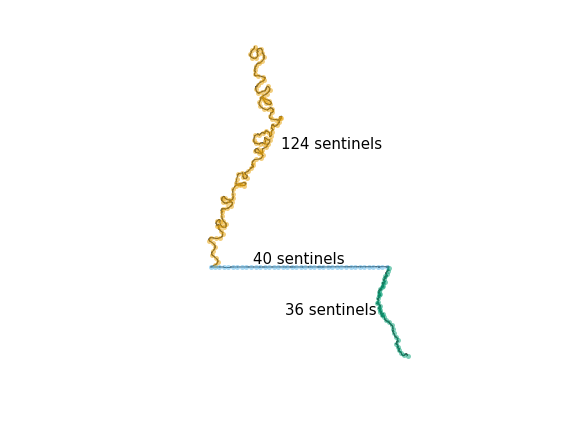
\includegraphics{figures/mississippi_counts.png}
\caption{mississippi counts}
\end{figure}

Secondly, the unweighted mean treatment estimand is affected by the
shape of the border between the treatment and control regions. We
illustrate this with the border separating two American States:
Louisiana and Mississippi. From North to South, the border follows the
meandering Mississippi river, then takes a sharp turn to the East and
becomes a straight line, until it meets the even more sinuous Pearl
river, which it then follows until it reaches the Gulf of Mexico.
Sentinels placed at constant intervals along this interval will
therefore be most densely packed along the Pearl River, and sparsest
along the straight segment of the border (see Figure
\ref{fig::mississippi_counts}). When averaging a function over the
border, those sections will therefore be overrepresented. Troublingly,
the sinuousness of the border therefore determines the estimand, and the
resolution of our map can drastically change our estimate, even though
the outcomes of the treatment we are studying might have nothing to do
with river topographies.

Weighing the treatment effect at each sentinel location by a local
density estimate would address the first issue, but not the second. We
view the unwelcome dependence of the \(\linavg\) estimand on the border
topography as a side effect of ignoring the fact that the 1-dimensional
treatment function \(\tau(\boundary)\) is embedded in a Euclidean
2-dimensional space. This fact is captured by the covariance structure:
sentinels in the straight segment of the border will be less strongly
correlated than in the sinuous segments. The more correlated sentinels
individually carry less information about the local treatment effect.
This suggests that instead of averaging the treatment effect evenly
along the border, we wish to average evenly the information contained
therein. This motivates the use of the inverse-variance weighted mean
\(\invvar\), which efficiently extracts the information from the
posterior to produce the weighted avereage with minimum variance.

\begin{align}
    \invvar \mid Y_T, Y_C, \sigmaf, \sigman, \ell &\sim \normal\del{\mu_{\invvar \mid Y}, \Sigma_{\invvar \mid Y}} \\
    \mu_{\invvar \mid Y} &\approx \del{\ones\trans \Sigma_{\sentinels \mid Y}^{-1} \mu_{\sentinels \mid Y}} \big/ \del{\ones\trans \Sigma_{\sentinels \mid Y}^{-1} \ones}  \\
    \Sigma_{\invvar \mid Y} &\approx 1 \big/ \del{\ones\trans \Sigma_{\sentinels \mid Y}^{-1} \ones} 
    \label{eq:invvar}
\end{align}

This estimator will automatically give more weight to sentinels in dense
areas (as the variance will be lower there), and to sentinels in
straight sections of the border. While the estimand is less clear, the
approach is in keeping with the philosophy of regression discontinuity
designs. We let information be our guide when averaging over our
boundary, just like it guided the analysis of regression discontinuity
designs to only focus on the treatment effect at the boundary. The
estimand isn't chosen by the scientist, but it is dictated by the
limitations of the data.
    


    	\section{Spatial advantage}\label{spatial-advantage}

\begin{itemize}
\tightlist
\item
  spreading units along a boundary doesn't necessarily reduce power
\item
  multiple experiments interpretation
\end{itemize}

Classical regression discontinuity designs often suffer from low power,
requiring many units near the boundary for inference to be possible. In
the spatial RDD setting, we might worry that the situation is worse, as
geographical datasets with many units packed along the boundary are
uncommon. In geographical settings, each unit (e.g.~household or
counties) normally takes up space, so there is a limit to how densely
packed units can be near the boundary. And boundaries often include
sparsely populated segments, e.g.~running through parks, industrial
areas, or farmland. The intuition that spatial RDDs will therefore
suffer from low power is correct, inasmuch as at any given point along
the boundary, the posterior variance of \(\tau(\boundary)\) will
typically be high. But once we pool the information into an average
treatment effect, or perform a sharp test, spatial RDDs can be more
powerful than classical RDDs, with the same number of units at the same
distance from the boundary.

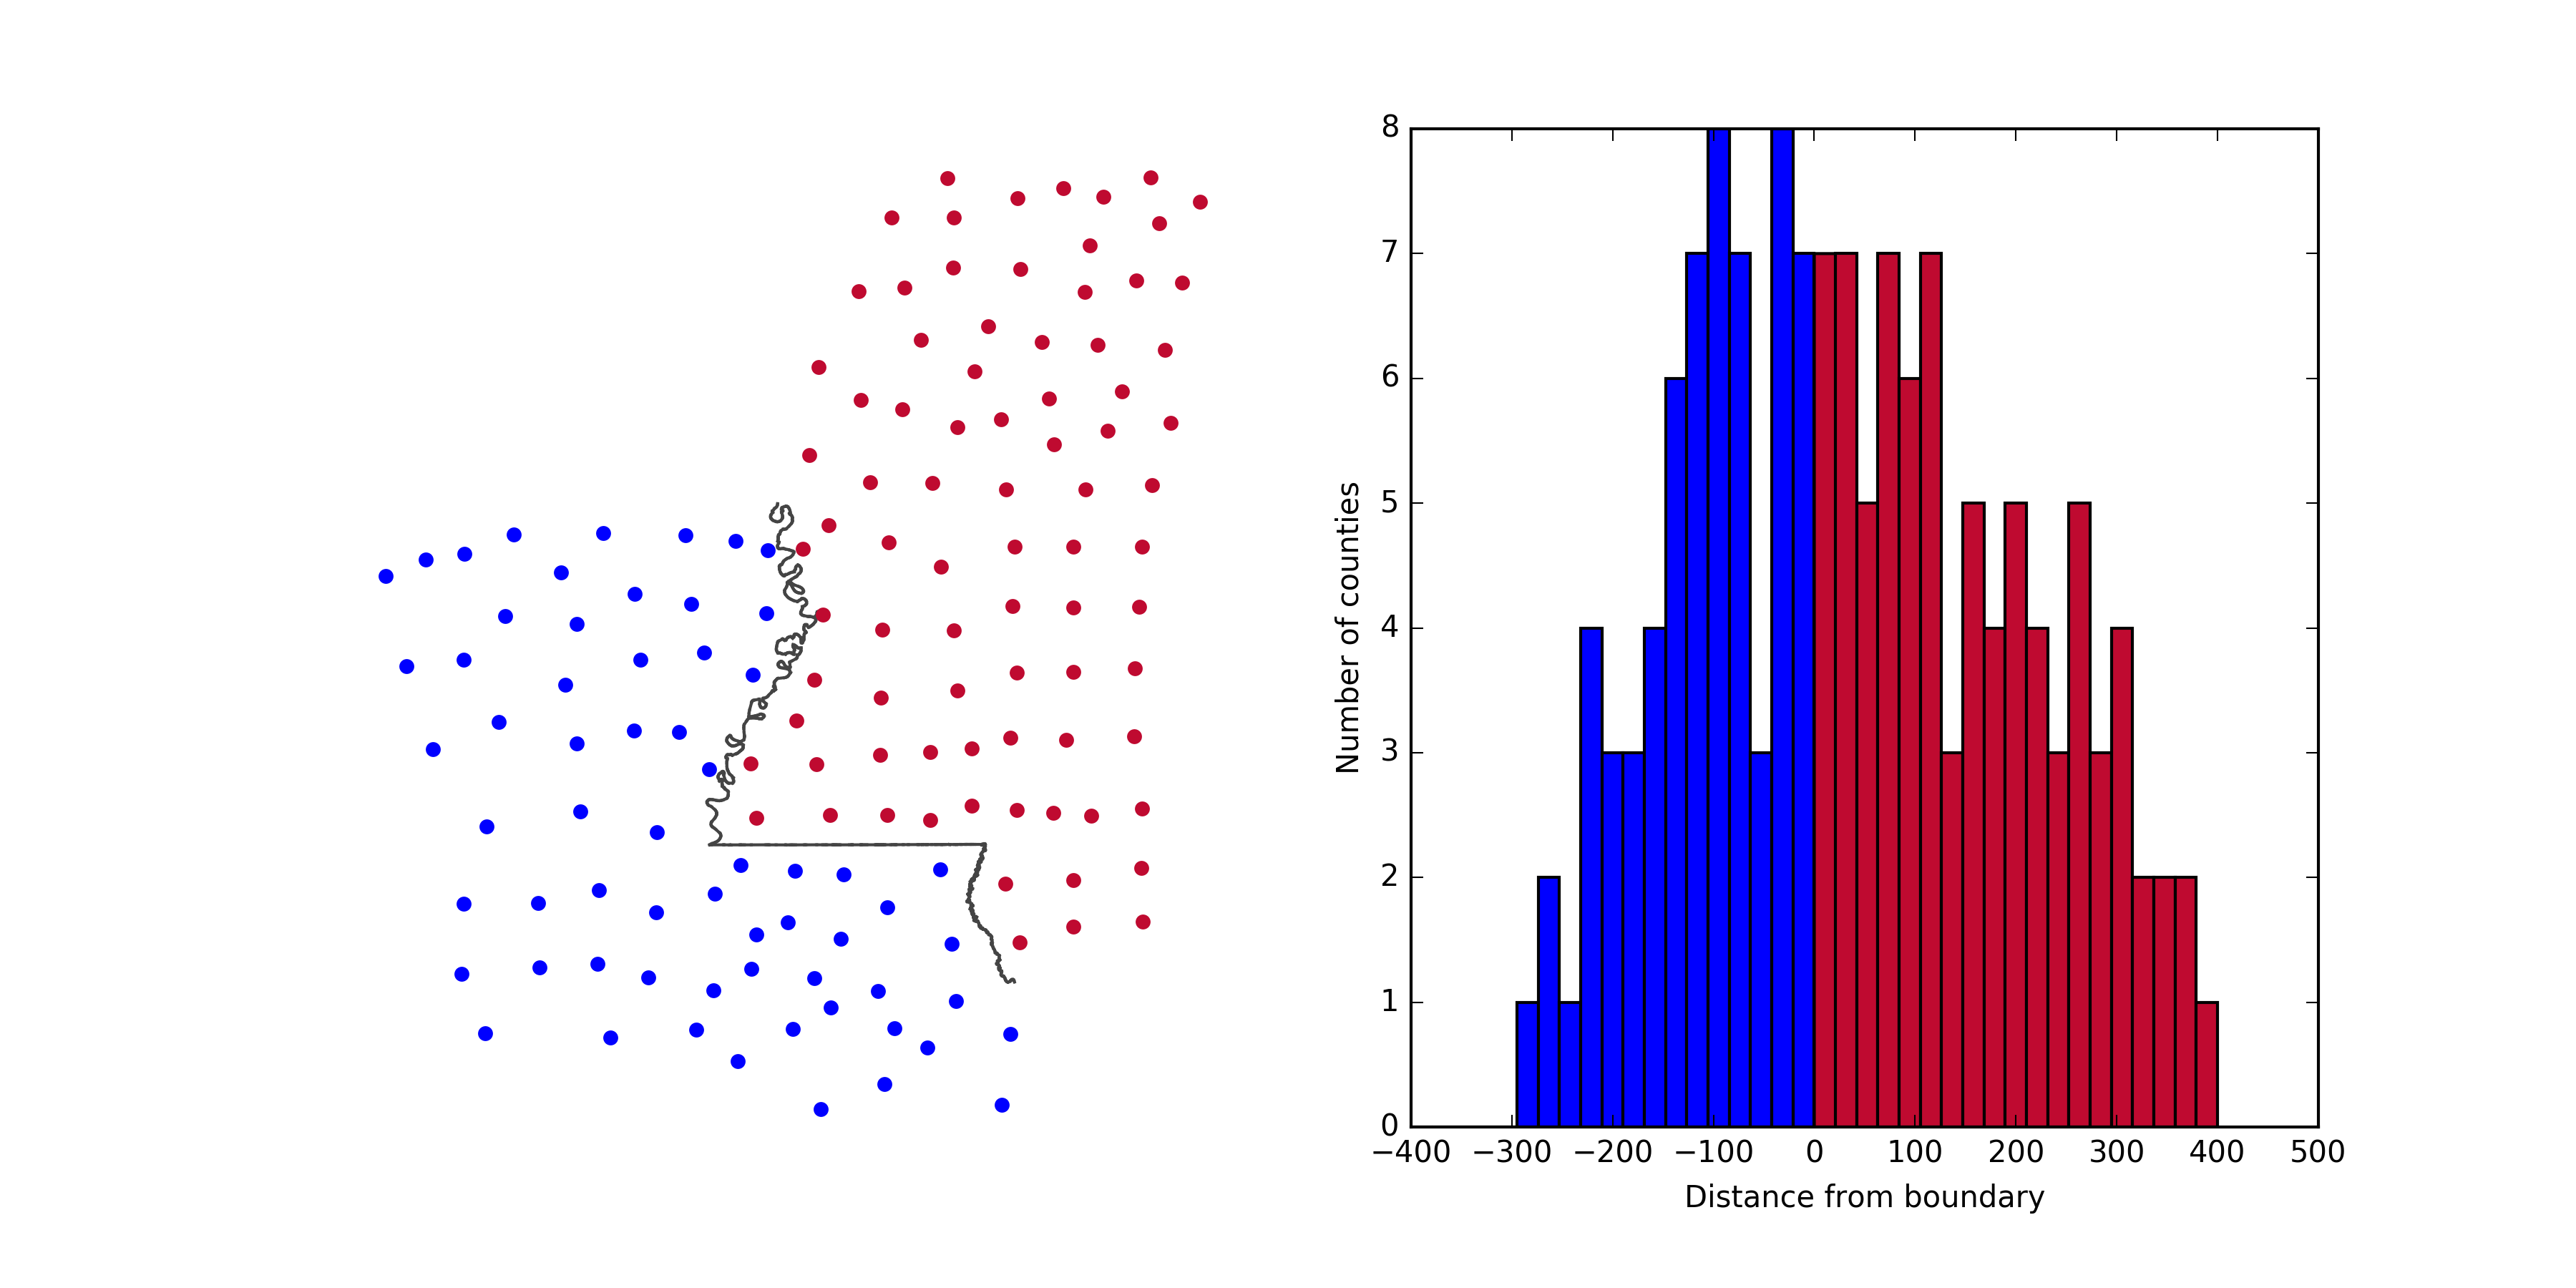
\includegraphics{figures/mississippi_counties.png}
\(\label{fig:mississippi_counties}\)

We illustrate this statement with an example. Considering once more the
boundary between Louisiana and Mississippi, we imagine an experiment
where the unit of analysis is the county, located at its centroid, as
shown in Figure \ref{fig:mississippi_counties}(a). For simplicity, we
fix the hyperparameters to arbitrary values: \(\sigman=\sigmaf=1.0\) and
\(\ell=50\,\mathrm{km}\). The variance of the inverse-variance weighted
treatment effect \(\invvar\) is thence only a function of the positions
of the units, available analytically by plugging the posterior variance
\eqref{eq:postvar2gp} into the inverse-variance estimator
\eqref{eq:invvar}. Following this procedure, we obtain a posterior
standard deviation of the average treatment effect of 0.31. We then
create a one-dimensional regression discontinuity design for the same
setting, by using each unit's distance from the boundary as the
covariate \(x\), the distribution of which is shown in Figure
\ref{fig:mississippi_counties}(b). Following the exact same 2GP
procedure with the same hyperparameters as in the spatial setting, and
with a discontinuity at \(x=0\), we again compute the posterior standard
deviation of the treatment effect at the boundary (now a single number
rather than a continuous function) , this time obtaining 0.58. This
higher figure indicates that, perhaps counter-intuitively, the spatial
experiment actually has more power than its one-dimensional analog.

To gain intuition about the higher power of the spatial RDD, we turn to
the interpretation of regression discontinuity designs as natural
experiments {[}need reference{]}. Near the discontinuity, we can
reasonably claim that the side of the discontinuity that each unit fell
into was largely dictated by random noise in the covariate. This in turn
allows us to claim that a natural randomized experiment took place near
the boundary, with treatment and control units coming from the same
population. We can extend this interpretation to the spatial setting, by
conceiving of multiple correlated experiments taking place all along the
boundary. The average treatment effect estimator then pools the
information supplied by all of these experiments. The question then
becomes: do we get more powerful inference by grouping all the units
into a single experiment, or by spreading them along a multitude of
weaker experiments? There are two sources of uncertainty in our model:
the observation noise \(\epsilon_i\), and the underlying processes
\(g_T\) and \(g_C\). Adding more units to a single experiment allows us
to cancel out more of the observation noise, but if the new units aren't
added closer to the discontinuity, uncertainty always remains in \(g_T\)
and \(g_C\). In the spatial setting, however, we observe multiple
realizations of the Gaussian process, and therefore do not suffer from
the same diminishing returns.
    


    	\section{Example: NYC school
districts}\label{example-nyc-school-districts}

\section{Conclusion}\label{conclusion}
    



    % Add a bibliography block to the postdoc
    
    
    
    \end{document}
